\documentclass[12pt,a4paper]{scrartcl}
\usepackage[utf8]{inputenc}
\usepackage[ngerman]{babel}
\usepackage{amsmath,amssymb,amstext}
\usepackage{fancyhdr}
\usepackage{trsym,trfsigns}
\usepackage{graphicx}
\title{Integraltransformation}
\subtitle{Zusammenfassung}
\author{Grasso Antonino}
\date{Sommersemester 21}

\pagestyle{fancy}
\fancyhf{}
% Header
\lhead{Integraltransformation}
\rhead{Zusammenfassung}
% Footer
\cfoot{Grasso}
\rfoot{\thepage}

\begin{document}

% Title
\begin{titlepage}
\maketitle
\vspace{100px}

\end{titlepage}

% Table of contents
\tableofcontents
\newpage

% Content

\section{Verlauf und Rahmen}
\label{sec:verlauf-und-rahmen}
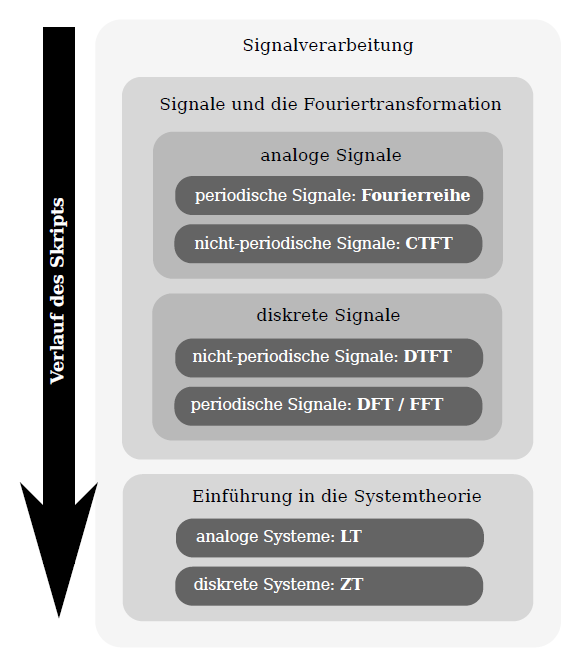
\includegraphics[height=10cm]{Pictures/Verlauf.png}

\section{Klassifizierung von Signalen}
\label{sec:klassifizierung}
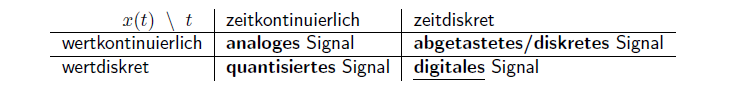
\includegraphics[height=2cm]{Pictures/Einheiten.png}

\section{Definitionen und Konstanten}
\label{sec:definitionen-und-konstanten}

\subsection{Funktionen}
\label{sec:sub:funktionen}
\subsubsection{sinc-Funktion $sinc(t)$}
\label{sec:sub:sub:sinc-funktion}
$$sinc(t) = \frac{\sin(t)}{t}$$
\subsubsection{Sprungfunktion $\varepsilon(t)$}
\label{sec:sub:sub:sprungfunktion}
$$\varepsilon(t) := $$ 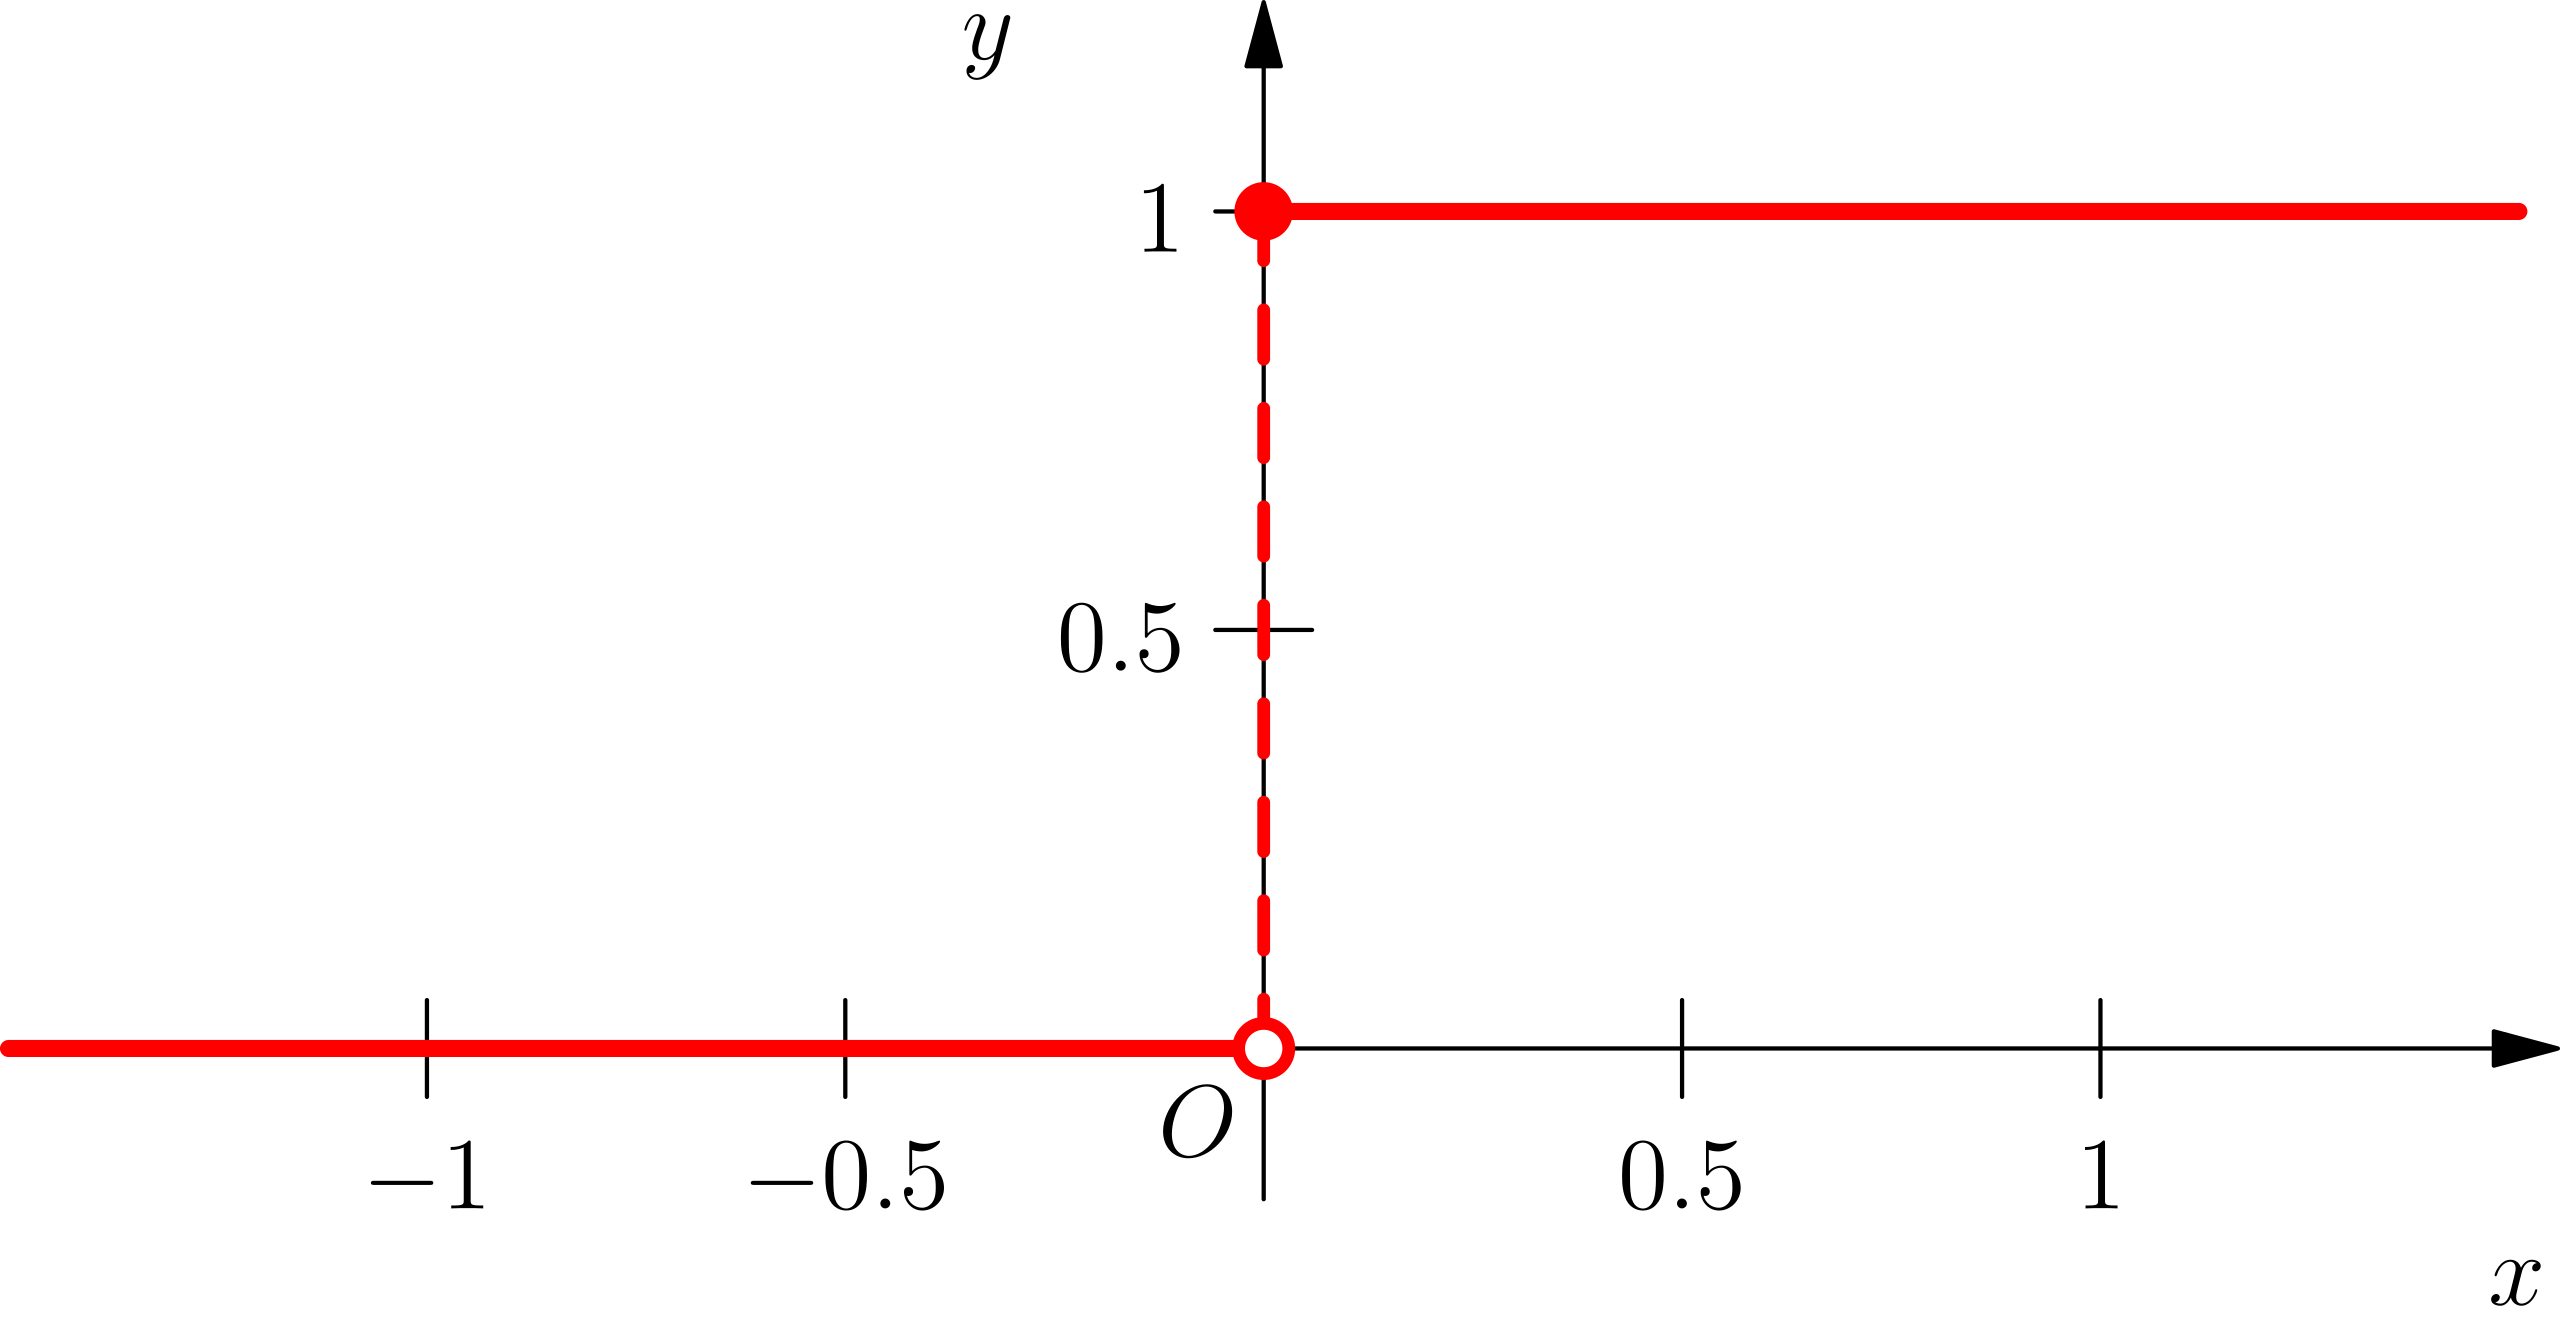
\includegraphics[height=5cm]{Pictures/Heaviside.svg.png}
\subsubsection{Zeitsignal $x(t)$}
\label{sec:sub:sub:zeitsignal}
$$x(t) := Zeitsignal$$
\subsubsection{Frequenzspektrum $X(\omega)$}
\label{sec:sub:sub:frequenzspektrum}
$$X(\omega) := Frequenzspektrum $$
\subsubsection{Abgetastetes Zeitsignal $x_A(t)$}
\label{sec:sub:sub:abgetastetes-zeitsignal}
$$x_A(t) := abgetastetes\ Zeitsignal$$
\subsubsection{Abgetastetes Frequenzspektrum $X_A(\omega)$}
\label{sec:sub:sub:abgetastetes-frequenzspektrum}
$$X_A(\omega) := abgetastetes\ Frequenzspektrum $$

\subsection{Analoge Signale}
\label{sec:sub:const-def-analoge-signale}
\subsubsection{Periodendauer $T_p$}
\label{sec:sub:sub:periodendauer}
$$ x(t) := \mathbb{R} \to \mathbb{R}$$
$$T_p := x(t + n \cdot T_p) = x(t)$$
\subsubsection{Frequenz $f$}
\label{sec:sub:sub:frequenz}
$$f = \frac{1}{T_p} = \frac{\omega_p}{2\pi}$$
\subsubsection{Kreisfrequenz $\omega_p$}
\label{sec:sub:sub:periodendauer-im-spektrum-kreisfrequenz}
$$\omega_p = \frac{2\pi}{T_p}$$
\subsubsection{Bandbreite $B$}
\label{sec:sub:sub:bandbreite}
$$B :=$$ höchste vorkommende Frequenz

\subsection{Diskrete Signale}
\label{sec:sub:const-def-diskrete-signale}

\subsubsection{Abtastfrequenz $f_A$}
\label{sec:sub:sub:abtastfrequenz}
$$f_A = \frac{1}{\Delta T_A} = \frac{\omega_p}{2\pi}$$

\subsubsection{Blocklänge $N$}
\label{sec:sub:sub:blocklaenge}
$$N :=$$ Anzahl an Stellen des diskreten Signals
$$T_A \cdot \omega_P = 2\pi \cdot N$$ Das Produkt aus Periodendauern ist eine konstante Grösse, welche sich nur mit der Blocklänge N verändern lässt.\\
$\to$ Unschärferelation der DFT (1. Variante)
$$\Delta T_A \cdot \Delta \omega_P = \frac{2\pi}{N}$$ Das Produkt der Abtastabstände ist ebenso eine konstante Grösse, welche sich nur durch Blocklänge N verändern lässt.\\
$\to$ Unschärferelation der DFT (2. Variante)

\subsubsection{Zeitabstände $\Delta T_A$}
\label{sec:sub:sub:delta-t-a}
$$\Delta T_A :=$$ Zeitabstände der Abtastung im Zeitraum

\subsubsection{Frequenzabstände $\Delta \omega_p$}
\label{sec:sub:sub:delta-omega-p}
$$\Delta \omega_p :=$$ Frequenzabstände der Abtastung im Frequenzspektrum \\
$$\Delta \omega_P = \frac{2\pi}{T_A} \Rightarrow$$ Länge der Periode im Zeitraum legt Feinheit der Abstastung im Frequenzraum fest.

\subsubsection{Periodendauer im Zeitraum $T_A$}
\label{sec:sub:sub:t-a}
$$T_A = N \cdot \Delta T_A :=$$ Periodendauer im Zeitraum $=$ Signaldauer

\subsubsection{Periodendauer im Frequenzspektrum $\omega_p$}
\label{sec:sub:sub:omega-p}
$$\omega_p = N \cdot \Delta \omega_P :=$$ Periodendauer im Frequenzraum $=$ max. Signalfrequenz\\
$$\omega_p = \frac{2\pi}{\Delta T_A} \Rightarrow$$ Die Feinheit der Abtastung im Zeitraum legt die maximale angenommene Frequenz fest $\to$ Abtasttheorem!

\newpage
\section{Signale und Fouriertransformation}
\label{sec:signale-und-fouriertransformation}

\subsection{Analoge Signale}
\label{sec:sub:analoge-signale}

\subsubsection{Fourierreihe (analoge, periodische Signale)}
\label{sec:sub:sub:fourier-reihe}

Jedes Signal $x(t)$ kann als unendliche Summe von überlagerten Sinus und Cosinus Funktionen dargstellt werden: \\

\noindent  \textbf{Sinus-Cosinus-Darstellung der Fourierreihe:}
\begin{equation}
  \label{eq:1}
  \begin{split}
  x(t) &=\frac{a_0}{2} \sum_{n=1}^{\infty}\big(a_n \cdot \cos(n \omega_p t) + b_n \cdot \sin(n \omega_p t)   \big)  \\
a_n &= \frac{2}{T_p} \int_{-\frac{T_p}{2}}^{\frac{T_p}{2}} x(t) \cdot \cos(n\omega_p t)\ dt \\
b_n &= \frac{2}{T_p} \int_{-\frac{T_p}{2}}^{\frac{T_p}{2}} x(t) \cdot \sin(n\omega_p t)\ dt
    \end{split}
\end{equation}
\noindent $a_n$ und $b_n$ dienen hierbei als Ähnlichkeitsmass wie sehr sich die Ursprungsfunktion $x(t)$ der jeweiligen Elementarfunktion $\big(sin(n\omega_p t)$ oder $cos(n\omega_p t)\big)$ ähnelt.\\

\noindent \textbf{Bemerkungen:}
    \begin{itemize}
      \item Die Fourierreihe nimmt an Sprungstellen den Mittelwert von linksseitigem und rechtsseitigem Grenzwert an
      \item Zur Berechnung der Fourierkoeffizienten lässt sich das Integrationsintervall verschieben z.B. zu $(0,T_p)$. \\
    \end{itemize} 

    \noindent \textbf{Betrags-/Phasen-Darstellung der Fourierreihe:}
\begin{equation}
    \label{eq:2}
    \begin{split}
    x(t) &=\frac{A_0}{2} + \sum_{n=1}^{\infty} A_n \cdot \cos(n \omega_p t + \varphi_n)  \\
  A_n &= \sqrt{a^2_n + b^2_n} \\
  \varphi_n &= -\arctan\bigg(\frac{b_n}{a_n}\bigg)
      \end{split}
  \end{equation}
  \noindent Diese Darstellung lässt sich aus den Additionstheoremen von Sinus und Cosinus ableiten. \\

  \noindent \textbf{Komplexe Darstellung der Fourierreihe:}
  \begin{equation}
    \label{eq:3}
    \begin{split}
    x(t) &= \sum_{n= -\infty}^{\infty} c_n e^{jn\omega_p t}\\
    c_n &= \frac{1}{T_p} \int_{-\frac{T_p}{2}}^{\frac{T_p}{2}} x(t) \cdot e^{-jn\omega_p t}\ dt
    \end{split}
  \end{equation}
  \noindent Herleitung: \\
  Mit 
  $$e^{j\omega t} := \cos(\omega t) + j\cdot \sin(\omega t)$$ erhält man $$\cos(\omega t) = \frac{1}{2}(e^{j\omega t} +  e^{-j\omega t})$$ 
  und daher:
  $$\frac{A_0}{2} + \sum_{n=1}^{\infty} A_n \cdot \cos(n \omega_p t + \varphi_n) =  \sum_{n=0}^{\infty}c_n e^{jn\omega_p t} +  \sum_{n=1}^{\infty}c_{-n}e^{-jn\omega_p t}$$
  $$c_n = \frac{A_n}{2} e^{j\varphi_n}$$
  $$ c_{-n} = \frac{A_n}{2} e^{-j\varphi_n}$$ 

  \noindent \textbf{Umformungen:}\\
  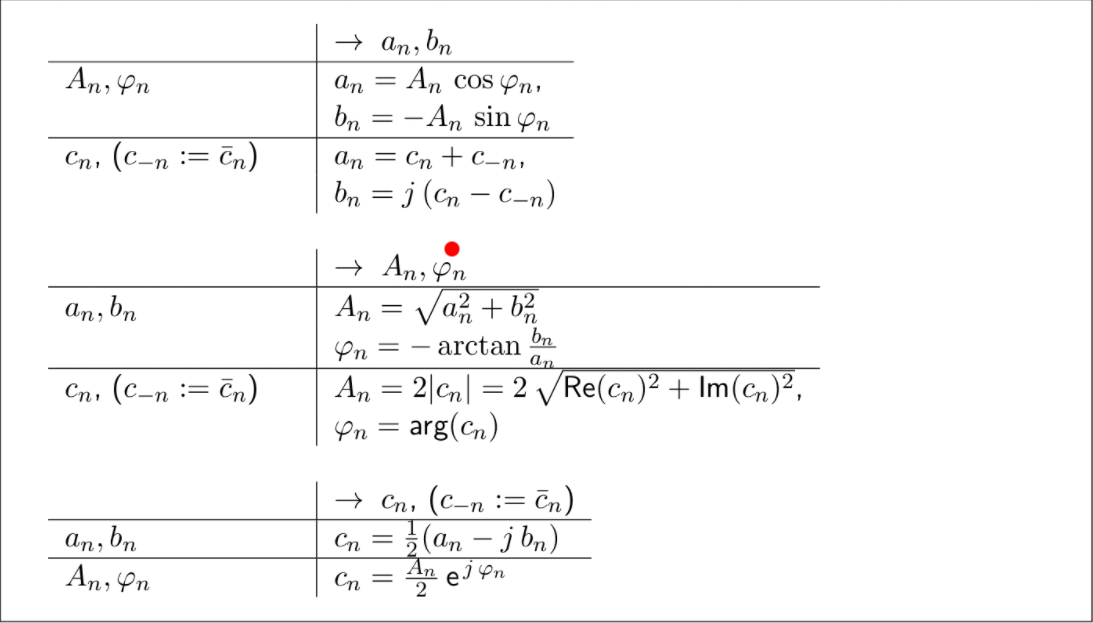
\includegraphics[height=6cm]{Pictures/Umformung.png} \\

  \noindent \textbf{Bedingungen für die Transformation:} 
  \begin{itemize}
  \item Die Funktion muss periodisch sein.
  \item  Innerhalb einer Periode aufteilbar in endlich viele stetige Teilstücke.
  \item Es dürfen keine divergierende Sprungstellen auftauchen.
  \end{itemize}

  \subsubsection{CTFT (analoge, nicht-periodische Signale)}
  \label{sec:sub:sub:ctft}

  \noindent Der Sinn der CTFT: Man möchte vom Zeitsignal $x(t)$ zum Frequenzspektrum $X(\omega)$. \\
  \noindent Die Idee der CTFT: Man nimmt die Fourierreihe und lässt $T_p \to \infty$ gehen: \\
  \begin{equation}
    \label{eq:4}
      \begin{split}
      X(\omega) &= \int_{-\infty}^{ \infty} x(t) \cdot e^{-j \omega t}\ d t\ (CTFT/FT) \ (aus\ 5) \\
      x(t) &= \frac{1}{2\pi} \int_{-\infty}^{ \infty} X(\omega) \cdot e^{j \omega t}\ d \omega\ (ICTFT/IFT) \ (aus\ 6) 
      \end{split}
    \end{equation}
 \noindent   Herleitung:\\
  \noindent Wir definieren eine Hilfsvariable: $\omega_n = n\omega_p$, sodass gilt:
  $\omega_{n+1} - \omega_n = \omega_p = \frac{2\pi}{T_p}$ und beginnen mit:
  $$x(t) = \sum_{n=-\infty}^{\infty} c_n e^{j \omega_n t}$$
  und
  $$c_n := \frac{1}{T_p}\int_{-\frac{T_p}{2}}^{\frac{T_p}{2}}x(t) \cdot e^{-j \omega_n t}\ dt$$

  \noindent Wir definieren eine Funktion in Abhängigkeit von $\omega_n$:
  \begin{equation}
  \label{eq:5}
    \begin{split}
    X(\omega_n) &:= \frac{2\pi}{\omega_p}c_n\ \ \big( \Leftrightarrow c_n = \frac{\omega_p}{2\pi}X(\omega_n)\big)\\
    &= \int_{-\frac{T_p}{2}}^{\frac{T_p}{2}}x(t) \cdot e^{-j \omega_n t}\ d t
    \end{split}
  \end{equation}

  \noindent Das neu gewonnene $c_n$ wird nun als Koeffizient in die ursprüngliche komplexe Fourierreihe eingesetzt:
  \begin{equation}
    \label{eq:6}
      \begin{split}
      x(t) &= \sum_{n=-\infty}^{\infty}\frac{\omega_p}{2\pi}X(\omega_n)e^{j\omega_n t}\\
      &= \frac{1}{2\pi} \sum_{n=-\infty}^{\infty} X(\omega_n) e^{j\omega_n t} \omega_p \\
      &= \frac{1}{2\pi} \sum_{n=-\infty}^{\infty} X(\omega_n) e^{j\omega_n t} \ (\omega_{n + 1} - \omega_n)  \\
      \end{split}
    \end{equation}
    \noindent Lässt man nun $T_p \to \infty$ gehen, wird $\omega_p$ immer kleiner und die Unterteilungen $\omega_n$ wandern dichter zueinander
    und im Grenzfall ein kontinuierlicher Verlauf $(\omega_ n \to \omega)$ und man erhält ein Riemann-Integral. Daraus folgert sich die oben aufgeführten Integrale für $x(t)$ und $X(\omega)$.\\

    \noindent  \textbf{Bemerkungen:}
    \begin{itemize}
      \item Stärke des Vorhandenseins einer Frequenz: $|X(\omega)|$
      \item Verschiebung der einzelenen Frequenzen: $\varphi = \arg(X(\omega))$
      \item Es gilt: $\overline{X(\omega)} = X(-\omega)$
      \item Bei reellen Signalen ist Betragsspektrum $|X(\omega)|$ symmetrich um Null
    \end{itemize}

    \subsubsection{Einschub: Die kontinuierliche Faltung}
  \label{sec:sub:sub:faltung}

  \begin{equation}
    \label{eq:7}
      \begin{split}
      y(t) &:= x_1 (t) * x_2 (t) = \int_{-\infty}^{\infty} x_1 (\tau) \cdot x_2 (t-\tau)\ d \tau \\
      \end{split}
    \end{equation}
  
    \noindent (Integral)\\
    \noindent Mit der Laufvariable $\tau$ läuft man $x_1$ forwärts durch und $x_2$ rückwärts aber um $t$ verschoben durch. \\
    $t$ ist hier als fester, bekannter Wert zu interpretieren. \\

    \noindent(Faltung) (Man macht das was oben drüber steht für jedes beliebige $t$)\\
    \noindent Man legt ein $\tau$ für $x_1$ und $x_2$ fest, verändert $t$ laufend und sieht sich die Schnittfläche der beiden Funktionen an. \\

    \noindent Main Purpose in der Signalverarbeitung: Abschwächung / Auslöschung von hohen Frequenzen.

  \subsubsection{Einschub: Der Delta-Impuls}
  \label{sec:sub:sub:delta-impuls}

  \noindent Wir definieren eine Funktion:
  \begin{equation}
    \label{eq:8}
    \begin{split}
    \delta (t) &= 0\ \ for\ t \neq 0 \\    
    \int_{-\infty}^{\infty} \delta (t)\ d t &= 1
    \end{split}
    \end{equation}
  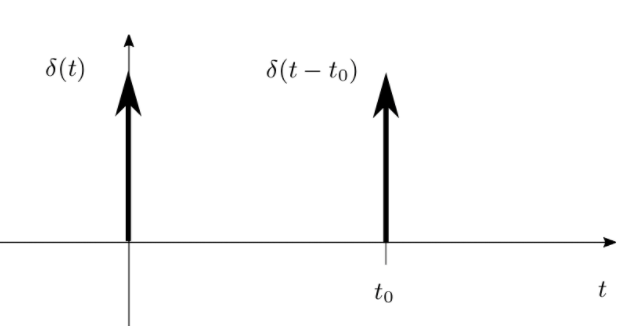
\includegraphics[height=4cm]{Pictures/DeltaImpuls.png} \\

  \noindent  \textbf{Verwendung des Delta-Impulses (Ausblendeigenschaft):}
  \begin{equation}
    \label{eq:9}
    \begin{split}
    \int_{-\infty}^{\infty} x(t) \cdot \delta(t-t_0)\ d t &= \int_{-\infty}^{\infty} x(t_0) \cdot \delta (t-t_0)\ d t \\    
    &= x(t_0) \cdot \int_{-\infty}^{\infty} \delta (t-t_0)\ dt \\
    &=x(t_0)
    \end{split}
    \end{equation}
    \noindent $x(t)$ wird überall ignoriert ausser an der Stelle an der $\delta(t-t_0) \neq 0$, d.h. bei $t = t_0$.\\
    Quasi eine Abtastung der Funktion $x(t)$ an Stelle $t_0$.\\

    \noindent \textbf{Fouriertransformation des Delta-Impulses:}
    $$\int_{-\infty}^{\infty} \delta(t) \cdot e^{-j\omega t}\ dt = \int_{-\infty}^{\infty} \delta(t) \cdot e^{-j\omega 0}\ dt = \int_{-\infty}^{\infty} \delta(t) = 1$$
    $$\delta(t) \TransformHoriz 1 $$ 
    Das Spektrum des Delta-Impulses enthält alle Frequenz mit Gewicht 1! \\

    \noindent \textbf{Die Stammfunktion des Delta-Impulses: $\varepsilon(t)$:}
    $$\varepsilon (t) = \int_{-\infty}^{t} \delta(\tau)\ d \tau \Leftrightarrow  \frac{d}{dt} \varepsilon (t) = \delta (t) $$

     \noindent \textbf{Fouriertransformation der Sprungfunktion:}
     $$\varepsilon(t) \TransformHoriz \pi \cdot \delta(\omega) + \frac{1}{j\omega} $$

  \subsubsection{Faltung mit dem Delta-Impuls}
  \label{sec:sub:sub:faltung-mit-delta-impuls}

  \begin{equation}
    \label{eq:10}
    \begin{split}
    x(t) * \delta(t-t_0) &= \int_{-\infty}^{\infty} x(\tau) \cdot \delta\big((t-t_0) - \tau\big)\ d \tau  \\
    &= \int_{-\infty}^{\infty} x(\tau) \cdot \delta \big(\tau -(t-t_0)\big)\ d \tau \\    
    &=x(t - t_0)
    \end{split}
    \end{equation}

\noindent    Kurz bedeutet das
    $$x(t) * \delta(t-t_0) = x(t-t_0)\ ,$$
    und für $t_0 = 0$
    $$x(t) * \delta(t) = x(t)\ .$$
    \noindent Der Delta-Impuls ist das Neutrale Element bezüglich der Faltung!

  \subsubsection{Besonderheiten der CTFT}
  \label{sec:sub:sub:besonderheiten-ctft}

  \noindent \textbf{Eigenschaften der CTFT:}\\
  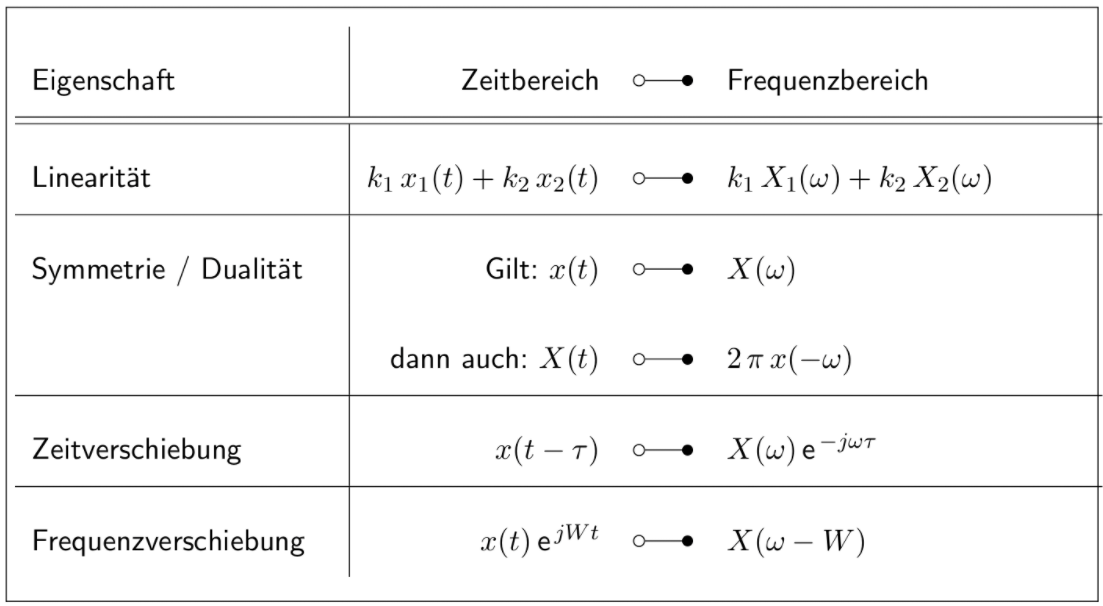
\includegraphics[height = 7cm]{Pictures/EigenschaftenCTFT.png}\\
  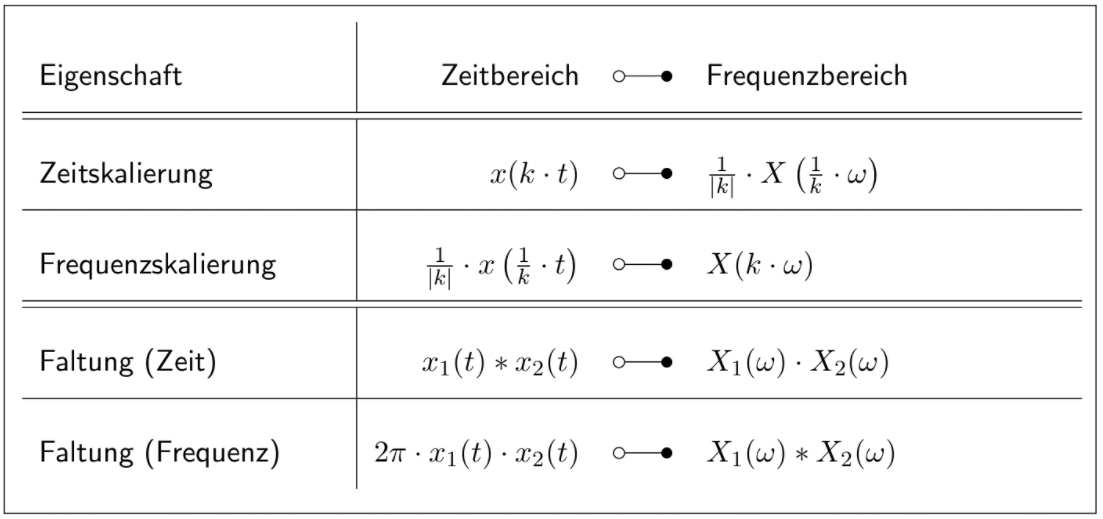
\includegraphics[height = 6cm]{Pictures/EigenschaftenCTFT2.png}\\
  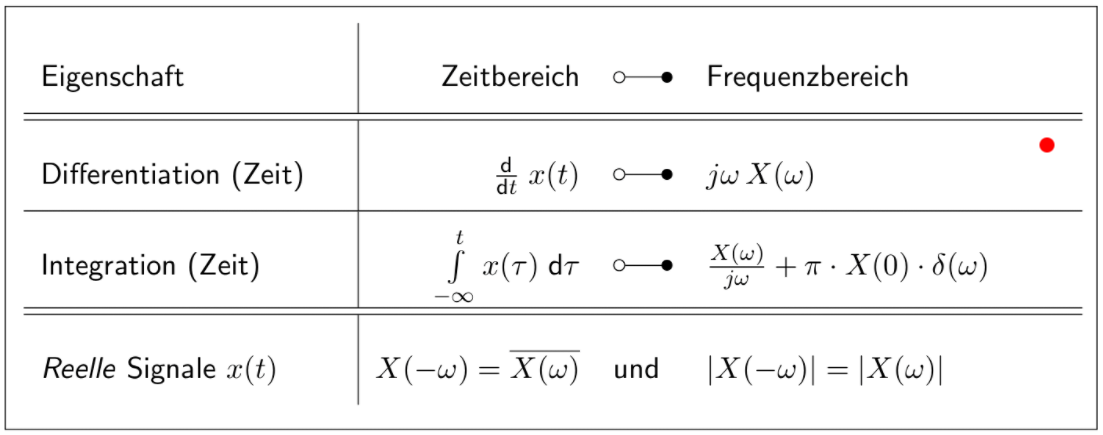
\includegraphics[height = 5cm]{Pictures/EigenschaftenCTFT3.png} \\

  \noindent \textbf{Signaldauer-Bandbreite-Produkt:}\\
  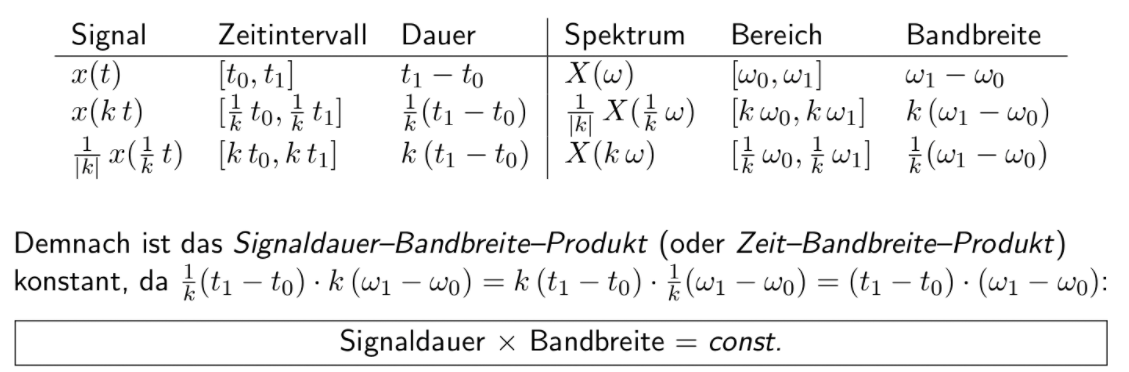
\includegraphics[height=5cm]{Pictures/SignalBand.png} \\

  \noindent \textbf{Korrespondenzen der CTFT:} \\
  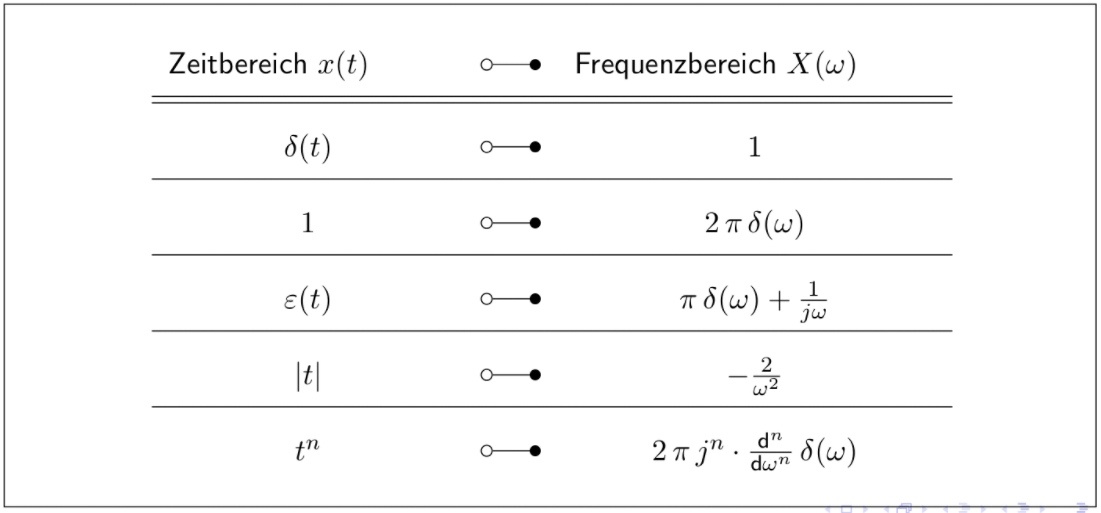
\includegraphics[height = 6cm]{Pictures/Korrespondenz.png}\\
  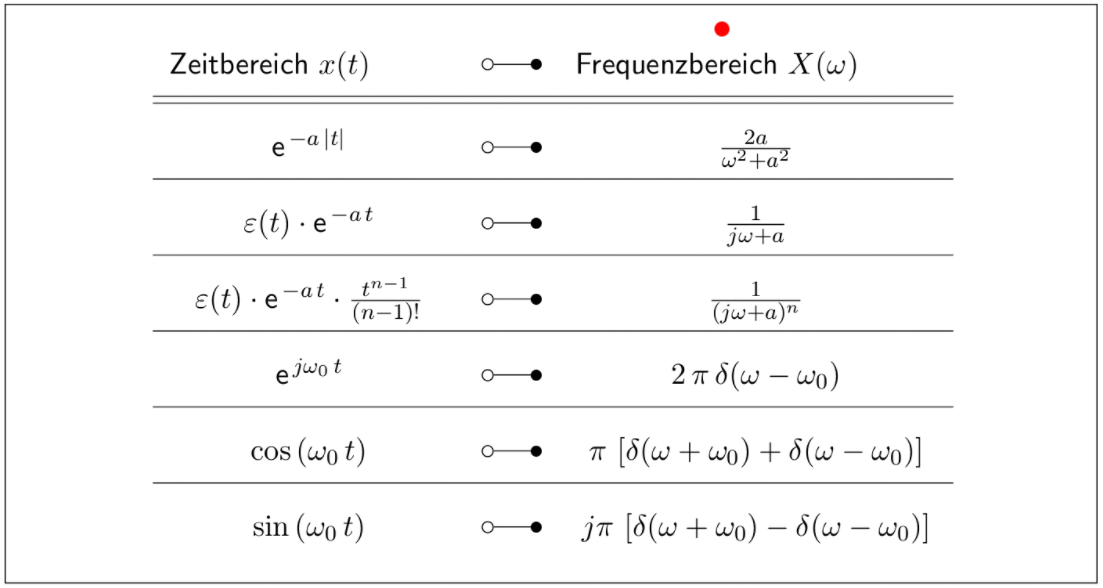
\includegraphics[height = 7cm]{Pictures/Korrespondenz2.png}\\
  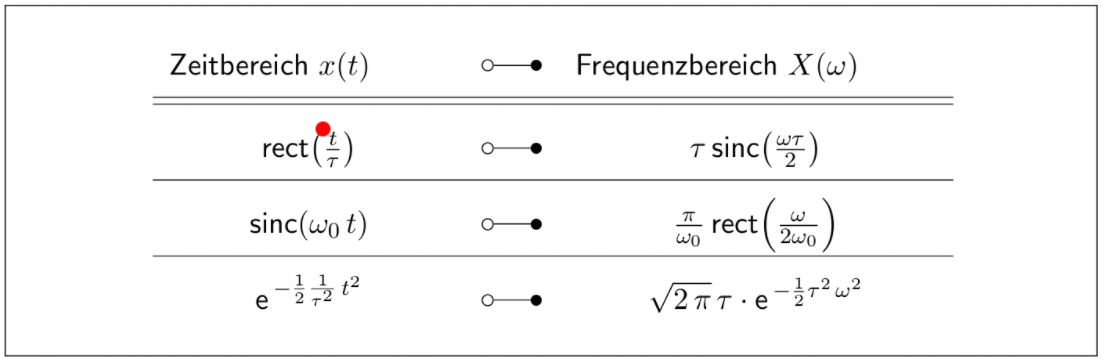
\includegraphics[height = 5cm]{Pictures/Korrespondenz3.png}

  \newpage
  \subsection{Diskrete Signale}
  \label{sec:sub:diskrete-signale}

  \subsubsection{Delta-Kamm}
  \label{sec.sub:sub:delta-kamm}
  \noindent Die Idee eines Delta-Kamms: Aus einer kontinuierlichen Funktion wird eine Zahlenfolge gemacht. \\
  
\noindent Um eine Zahlenfolge aus einer kontinuierlichen Funktion zu erhalten, muss diese abgetastet werden. 
Die Abtastung einer kontinuierlichen Funktion erfolgt mit einem Delta-Kamm:
  \begin{equation}
    \label{eq:11}
      \sum_{n = -\infty}^{\infty} \delta (t-n\Delta T_A)
  \end{equation}
\noindent Der Delta-Kamm stellt eine Schar einzelner Delta-Impulsen an bestimmten gewünschten Abtastungsorten mit gleichem Abstand voneinander dar: \\
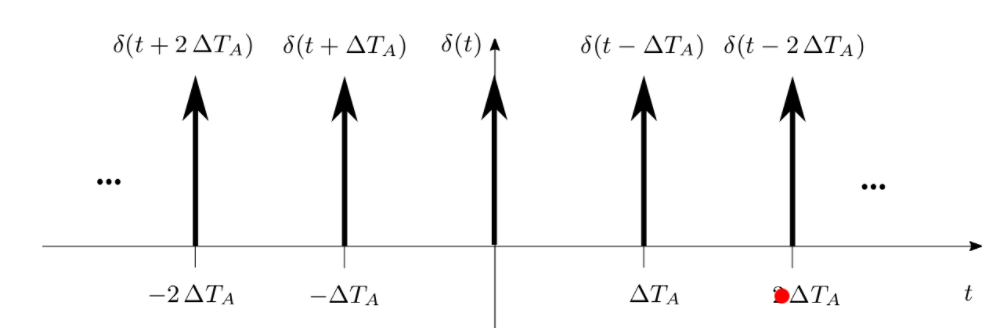
\includegraphics[height=5cm]{Pictures/DeltaKamm.png}

\subsubsection{Abgetastetes Signal}
  \label{sec.sub:sub:abgetastetes-signal}
\noindent Ein abgetastetes Signal ist mit Hilfe des Delta-Kamms definiert durch:
\begin{equation}
  \label{eq:12}
    x_A(t) := x(t) \cdot \sum_{n = -\infty}^{\infty} \delta (t-n\Delta T_A)
\end{equation} 
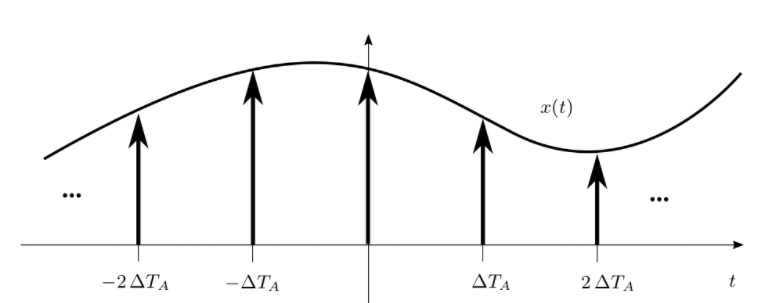
\includegraphics[height=5cm]{Pictures/AbgetastetSignal.png} \\
\noindent $x_A(t)$ wird auch als Diskretes Signal bezeichnet.

\subsubsection{DTFT (diskrete, nicht-periodische Signale)}
  \label{sec.sub:sub:dtft}

  \noindent Mit Hilfe der Ausblendeigenschaft des Delta-Impulses kann man die Fouriertransformation eines solchen abgetasteten Signals bestimmen:
  \begin{equation}
    \label{eq:13}
    \begin{split}
      X_A(\omega) &=  \int_{-\infty}^{\infty} x_A(t) \cdot e^{-j \omega t}\ d t \\
      &=  \int_{-\infty}^{\infty} x(t) \cdot \sum_{n = -\infty}^{\infty} \delta (t-n\Delta T_A) e^{-j \omega t}\ d t\\
      &= \sum_{n = -\infty}^{\infty} \int_{-\infty}^{\infty} x(t) e^{-j\omega t} \cdot \delta(t-n\Delta T_A)\ dt\\
      &= \sum_{n=-\infty}^{\infty} x(n\Delta T_A) e^{-j\omega n \Delta T_A}
    \end{split}
  \end{equation} 
  \\
  \noindent  \textbf{Bemerkungen:}
  \begin{itemize}
    \item Ein diskretes Zeitsignal führt dennoch zu einem kontinuierlichen Frequenzspektrum
    \item Durch Abtastung eines Zeitsignals mit Zeitabständen $\Delta T_A$ wird Frequenzspektrum periodisch mit Periodendauer $\omega_p:= \frac{2\pi}{\Delta T_A}$
    \item diskretes Zeitsignal $\TransformHoriz$ periodisches Spektrum
    \item periodisches Zeitsignal $\TransformHoriz$ diskretes Spektrum
    \item Zusammenhang CTFT und DTFT: $x_A(\omega) = \frac{1}{\Delta T_A} \sum_{ =-\infty}^{\infty} X\Big(\omega - \frac{2\pi n}{\Delta T_A}\Big)$
  \end{itemize}

  \subsubsection{Abtasttheorem}
  \label{sec.sub:sub:abtasttheorem}

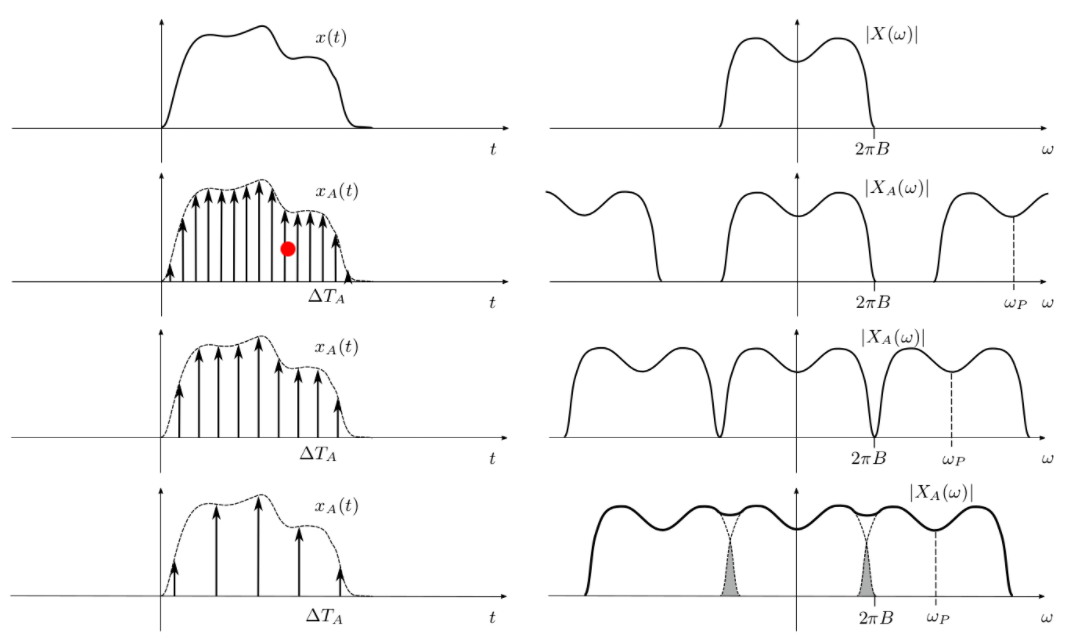
\includegraphics[height=9cm]{Pictures/Abtasttheorem.png} \\
\noindent Man folgert: $\omega_P > 2 \cdot 2\pi B$

\noindent Daraus ergibt sich das eigentliche Abtasttheorem:
\begin{equation}
  \label{eq:14}
  \begin{split}
    f_A = \frac{1}{\Delta T_A} > 2 \cdot B
    \Rightarrow \Delta T_A < \frac{1}{2 \cdot B}
  \end{split}
\end{equation} 

\noindent Ist das Abtasttheorem beim Abtasten eines Signales eingehalten, so kann versichert werden,
dass keine Informationen des Originalsignals verloren gehen und eine Rekonstruktion ist möglich.\\
$\Rightarrow$ "Mindestens mit der doppelt so grossen Frequenz wie im Originalsignal vorhanden ist abtasten." \\

\noindent  \textbf{Bemerkungen:}
  \begin{itemize}
    \item Die höchsten Frequenzen sind die, die zuerst unter der Verletzung des Abtasttheorems leiden (Unterabtastung)
    \item Informationsverlust ist nicht leicht zu beheben
    \item In der Praxis verwendet man häufig eine deutliche Überabtastung \\
  \end{itemize}

  \subsubsection{Rekonstruktion von abgetasteten Signalen}
  \label{sec.sub:sub:rekonstruktion-von-abgetasteten-signalen}

  \noindent   Unter der Annahme, dass das Abtasttheorem mit Zeitintervallen $\Delta T_A$ nicht verletzt wird,
  kann aus den diskreten Abtastwerten $x(n \Delta T_A)$ 
  die kontinuierliche Originalfunktion $x(t)$ rekonstruiert werden mit:
  \begin{equation}
    \label{eq:15}
    \begin{split}
     x(t) &:= \sum_{n=-\infty}^{\infty} x(n \Delta T_A) \cdot sinc\bigg(\frac{\pi}{\Delta T_A}(t-n\Delta T_A)\bigg)
    \end{split}
  \end{equation} 
  $\Rightarrow$ "Man interpoliert die diskreten Punkten mit der $sinc$-Funktion." \\

  \noindent Herleitung: \\
  \noindent 1. Schritt: Isolieren einer Periode durch Fenstern\\
  Man verwendet einen wichtigen Trick: Das sogenannte Fenstern von Signalen. \\
  Man multipliziert die periodische Fouriertransformierte des Abtastsignals $X_A(\omega)$ 
  mit einem Rechteckpuls der Breite $\omega_P$, 
  um die Fouriertransformierte des Originalsignals $X(\omega)$ zurück zu gewinnen:\\
  
  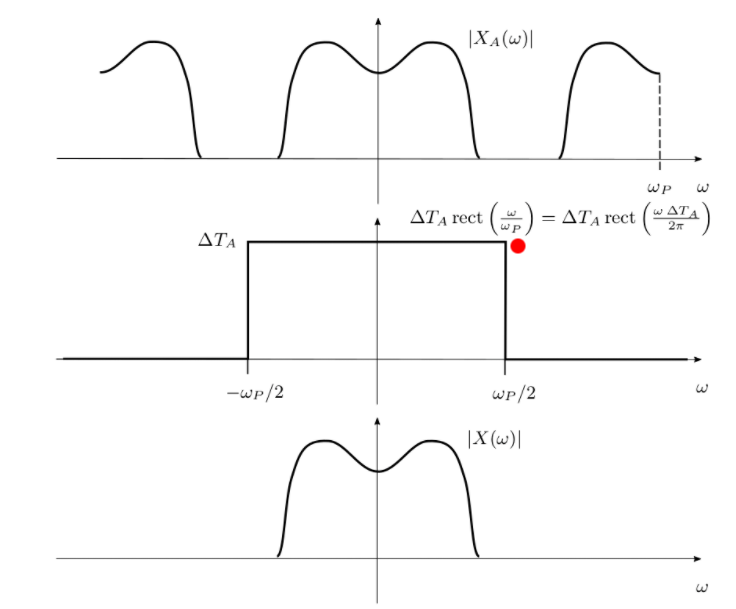
\includegraphics[height = 12cm]{Pictures/Fenstern.png}

  \noindent Signal Fenstern mathematisch: \\
  \begin{equation}
    \label{eq:116}
    \begin{split}
      X(\omega) &= X_A(\omega) \cdot \Delta T_A \cdot rect\bigg(\frac{\omega}{\omega_P}\bigg) \\
      &= X_A(\omega) \cdot \Delta T_A \cdot rect\bigg(\frac{\omega \Delta T_A}{2\pi}\bigg)
    \end{split}
  \end{equation} 

  \noindent 2. Schritt: Zurücktransformieren\\
  (Multiplikation im Spektrum $\Rightarrow$ Faltung im Zeitsignal)
  \begin{equation}
    \label{eq:17}
    \begin{split}
      X(\omega) &\TransformHoriz x_A(t) * sinc\bigg(\frac{t\pi}{\Delta T_A}\bigg) \\
        &= \int_{-\infty}^{\infty}x(\tau) \cdot \sum_{n=-\infty}^{\infty} \delta(\tau - n\Delta T_A) \cdot sinc\bigg(\frac{\pi}{\Delta T_A}(t-\tau)\bigg)\ d\tau \\
         &= \sum_{n=-\infty}^{\infty} \int_{-\infty}^{\infty}x(\tau) \cdot sinc\bigg(\frac{\pi}{\Delta T_A}(t-\tau)\bigg) \delta(\tau - n\Delta T_A)\ dt \tau \\
         &= \sum_{n=-\infty}^{\infty} x(n \Delta T_A) \cdot sinc\bigg(\frac{\pi}{\Delta T_A}(t-n\Delta T_A)\bigg) = x(t) 
        \end{split}
  \end{equation} 


  \subsubsection{DFT (diskrete, periodische Signale)}
  \label{sec.sub:sub:dft}

\noindent Der Sinn der DFT: Man will nicht nur das Signal auf einer digitalen Rechen- oder Speichereinheit verarbeiten, sondern auch das Spektrum. \\
  Die Idee der DFT: \\
    diskretes \& periodisches Zeitsignal $\TransformHoriz$ diskretes \& periodisches Spektrum \\
\begin{equation}
  \label{eq:18}
  \begin{split}
    X[m] = \sum_{n = 0}^{N-1} x[n]& e^{-j2\pi \frac{mn}{N}}\ (DFT) \\
    x[n] = \frac{1}{N}\sum_{m = 0}^{N-1} &X[m] e^{j2\pi \frac{mn}{N}}\ (IDFT) \\
    wobei& \\
    x[n] := x&(n\Delta T_A) \\
    X[m] := X&(m\Delta \omega_P)
  \end{split}
\end{equation}
\noindent Es gilt für Zeitsignal und Frequenzspektrum in dieser Darstellung die gleiche Periode N, d.h. $X[m+N] = X[m]$ und $x[m +N] = x[n]$. \\

\noindent  \textbf{Bemerkungen:}
  \begin{itemize}
    \item Man erhält für $N$ abgetastete Werte des Originalsignals automatisch auch $N$ Werte des Spektrums. 
    \item Zusammenhang diskretes Zeit- und Spektralsignal:\\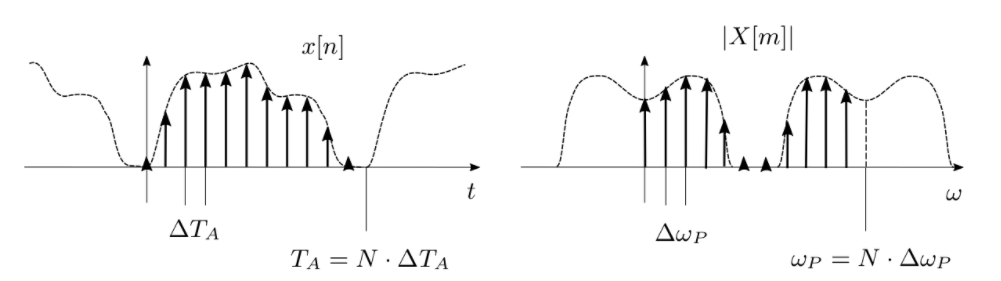
\includegraphics[height = 4cm]{Pictures/ZusammenhangN.png} 
    \item $X[N-m] = \overline{X[m]}$ und damit auch $|X[N-m]| = |\overline{X[m]}| = |X[m]|$
    \item Für ein reelles Signal x[n] ist das Betragsspektrum $|X[m]|$ immer symmetrich innerhalb einer Periode: $|X[m]| = |X[N-m]|$ für $m = 0,...,N-1$ \\
  \end{itemize}

 \noindent   Die Herleitung der DFT wird in 5. Schritten aufgeteilt: 
 \begin{itemize}
   \item Schritte 1-2: Erzeugen des diskreten und periodischen Zeitsignals für die DFT
   \item Schritte 3-5: Zusammenhang zwischen dem diskreten und periodischen Zeitsignal mit seinem diskreten und periodischen Spektrum 
   \item Der Zusammenhang wird durch folgende Argumentation erreicht: \\diskretes \& periodisches Zeitsignal $\TransformHoriz$ CTFT \{$\cdot$\} $\InversTransformHoriz$ ICTFT\{CTFT \{$\cdot$\}\}  
 \end{itemize}

 \noindent \\ 1. Schritt
 \begin{itemize}
   \item kontinuierliches Zeitsignal $x(t)$ im Intervall $[0, T_A]$ fenstern, so dass wesentliche Signalinformation enthalten ist.
   \item gefensterte Signal künstlich periodisch fortsetzen und umbenennen zu $x_P (t)$.
   \item Potentielle Fehler: Falsch abschneiden fürs zukünftige Periodisieren. \\$\to$ Leakage Fehler
 \end{itemize}
 
 \noindent \\ 2. Schritt
 \begin{itemize}
  \item Abtastung des periodischen Signals $x_P (t)$ wobei $N$ Abtastzeitpunkte im Grundintervall $[0, T_A]$ untergebracht werden. N wird als Blocklänge des diskreten Signals bezeichnet. 
  \item Dadurch haben die Abtastzeitpunkte einen Abstand von $\Delta T_A := \frac{T_A}{N}$. D.h. wir betrachten das abgetastete Signal: $$x_P (t) \cdot \sum_{n = -\infty}^{\infty} \delta(t - n \Delta T_A)$$
  \item Potentielle Fehler: Abtasttheorem verletzen.
\end{itemize}
\noindent\\ Grafik 1. und 2. Schritt:\\
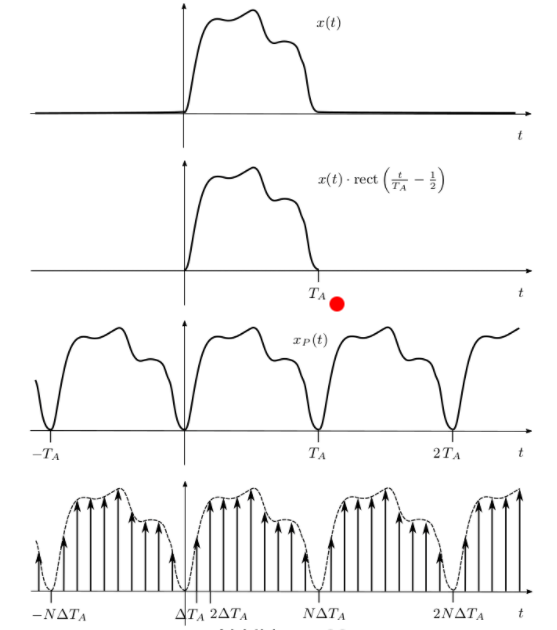
\includegraphics[height = 12cm]{Pictures/Schritt1.png}

\noindent \\ 3. Schritt | Konkrete Herleitung erspart
 \begin{itemize}
  \item Fouriertransformation (CTFT) für das abgetastete Signal: \begin{equation}
    \label{eq:19}
    \begin{split}
      & x_P (t) \cdot \sum_{n = -\infty}^{\infty} \delta(t - n \Delta T_A) \\
      \TransformHoriz & \Bigg[ \frac{2\pi}{N \Delta T_A} \sum_{n = 0}^{N -1} x(n \Delta T_A) e^{- j n\Delta T_A \omega} \Bigg] \cdot \Bigg[\sum_{k = -\infty}^{\infty} \delta(\omega - k\Delta \omega_p) \Bigg]
    \end{split}
  \end{equation}
  \item Es gilt im Grundintervall $[0, T_A]$, dass $x_p(n\Delta T_A) = x(n \Delta T_A)$.
  \item Es gilt im Grundintervall, dass die Konstante $\Delta \omega_p := \frac{2\pi}{N \Delta T_A}$ eingeführt wird.
  \item Wir stellen fest: Die Fouriertransformierte ist ein abgetastetes Signal mit Abtastorten $k\Delta\omega_p, k \in \mathbb{Z}$.
\end{itemize}

\noindent \\ 4. Schritt | Konkrete Herleitung erspart
 \begin{itemize}
  \item Inverse Fouriertransformation (ICTFT) auf das Spektrum, um wieder das Originalsignal an den Abtastorten zu erhalten: \begin{equation}
    \label{eq:20}
    \begin{split}
      \InversTransformHoriz & \Bigg[ \frac{1}{N} \sum_{k = 0}^{N -1} \sum_{n = 0}^{N -1}  x(n \Delta T_A) e^{- j 2\pi \frac{k n}{N}}e^{j2\pi \frac{k}{N} \frac{t}{\Delta T_A}} \Bigg] \cdot \Bigg[\sum_{l = -\infty}^{\infty} \delta(\omega - l\Delta T_A) \Bigg]
    \end{split}
  \end{equation}
  \item Die fordere eckige Klammer ist identisch zu $x_p(t)$.
  \item Ist $t \in [0,T_A]$, ist die fordere eckige Klammer sogar identisch zu x(t).
  \item Gilt auch für spezielle $t$: Für ein $t_0 \in [0,T_A] \Rightarrow x(t_0)$.
\end{itemize}

\noindent \\ 5. Schritt
 \begin{itemize}
  \item Die Erkenntnis von Schritt 4 für $t_0 = m\Delta T_A$ anwenden: 
  \begin{equation}
    \label{eq:21}
    \begin{split}
      x(m\Delta T_A) &= \frac{1}{N} \sum_{k = 0}^{N -1} \Bigg[ \sum_{n = 0}^{N -1}  x(n \Delta T_A) e^{- j 2\pi \frac{k n}{N}} \Bigg] e^{j2\pi \frac{km}{N} }
    \end{split}
  \end{equation}
  \item Die eckige Klammer $ =: X(k\Delta \omega_P)$ (DFT)
  \item Der ganze Ausdruck $ =:$ IDFT
\end{itemize}


\subsubsection{Handlungsanweisung zur DFT}
Dieser Abschnitt behandelt die konkrete Anwendung der DFT für z.B. eine Spektralanalyse oder digitale Filterung. \\
Man beginnt mit einem realen, kontinuerlichen Signal und will auch nach der DFT und IDFT dort wieder ankommen. \\

\noindent   Die Handlungsanweisung beinhaltet 7.Schritte:
 \begin{itemize}
   \item Schritte 1-3: Theoretischer Analog-Digital-Wandler.
   \item Schritte 4-6: Untersuchung (= Spektralanalyse) und Veränderung (= Filterung) des Spektrums. 
   \item Schritt 7: Theoretischer Digital-Analog-Wandler.
 \end{itemize}

 \noindent \\ \textbf{1. Schritt}
 \begin{itemize}
 \item Fenstern eines gegebenen kontinuierlichen Zeitsignal so passend, dass bei periodischer Fortsetzung keine künstliche plötzliche Störung des Signals auftritt.
 \item Dadurch wird $T_A$ festgelegt.
 \item Falsches fenstern führt zum Leakage Fehler \\(Sprünge im Zeitsignal $\to$ Falsche Frequenzen im Spektrum): \\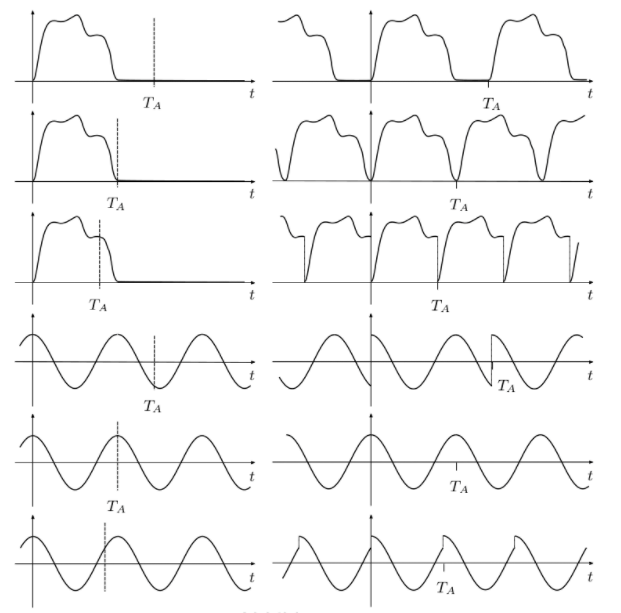
\includegraphics[height=10cm]{Pictures/BSPSchritt1.png} 
 \end{itemize}

 \noindent \\ \textbf{2. Schritt}
 \begin{itemize}
  \item Bestimmen der Blocklänge $N$, sodass das Abtasttheorem nicht verletzt wird. D.h. für ein bandbegrenztes Signal mit Bandbreite B ergibt sich dies zu: $$N \geq 2\ B\cdot T_A$$
  \item Hat man nun das beliebige $N$, kann man daraus die verwendete Abtastabstände bestimmen: $$ \Delta T_A = \frac{T_A}{N}$$
  \item Verletzung des Abtasttheorems führt zu Aliasing-Effekt \\(Unterabtastung $\to$ Misinformation): verweis auf \ref{sec.sub:sub:abtasttheorem} \\
 \end{itemize}

 \noindent \\ \textbf{3. Schritt}
 \begin{itemize}
  \item Abtasten des Signals zu den Zeitpunkten $t = n \Delta T_A,\ n = 0, .., N-1$ und es ergeben sich die diskreten Signalwerte: $$x[n] = x(n\Delta T_A)$$
 \end{itemize}

 \noindent \\ \textbf{4. Schritt}
 \begin{itemize}
  \item DFT durchführen:$$ X[m] = \sum_{n=0}^{N-1} x[n] e^{-j 2\pi \frac{mn}{N}},\ m= 0,..,N-1$$ an den Abtastorten $\omega_m = m\Delta \omega_P = m\frac{2\pi}{T_A},\ m= 0,..,N-1$.
 \end{itemize}

 \noindent \\ \textbf{5. Schritt}
 \begin{itemize}
  \item Betrachten und/oder verändern des Spektrums. Da die Veränderung (Filterung) des Spektrums eine so zentrale Rolle in der digitalen Signalverarbeitung spielt, wird aus dem gegbenen Spektrum X[m] ein neues Spektrum Y[m] erzeugt, bspw. durch Multiplikation einer Gewichtsfunktion $G$: $$Y[m] := G \cdot X[m], m = 0,..,N-1$$
 \end{itemize}

 \noindent \\ \textbf{6. Schritt}
 \begin{itemize}
  \item IDFT durchführen, um das gefilterte, diskrete Zeitsignal zu erhalten: $$ y[n] = \frac{1}{N} \sum_{m=0}^{N-1} Y[m]e^{j2\pi\frac{mn}{N}},\ n = 0,..N-1$$
  \item In vielen Anwendungen der digitalen Signalverarbeitung hört man hier auf, wenn man sich nicht für eine kontinuierliche Version des gefilterten Signals interessiert, sonst Rekonstruktion.
 \end{itemize}

 \noindent \\ \textbf{7. Schritt}
 \begin{itemize}
  \item An Schritt 6 anknüpfend kann man mit der Rekonstruktionsformel aus dem diskreten Signal die kontinuierliche, periodische Signalrekonstruktion bestimmen: $$y_p(t) = \sum_{n = -\infty}^{\infty} y[n] \cdot sinc \bigg(\frac{\pi}{\Delta T_A} ( t- n\Delta T_A)\bigg)$$
  \item Praktisch kann die undendliche Summe durch eine endliche Summe angenähert werden.
  \item Gute Annäherung: $$\sum_{n = -N+1}^{2N-2}$$
 \end{itemize}

 \noindent  \\ \textbf{Zero-Padding}
 \begin{itemize}
   \item Beliebtes Mittel bei gegebenen Abtastabständen $\Delta T_A$ eine feinere Abtastung des Spektrums zu erreichen ist das $zero-padding$: $x[n]$ mit Nullen füllen
   \item Blocklänge $N$ und Signaldauer $T_A$ werden so künstlich vergrössert. 
   \item $\Delta \omega_P$ wird so automatisch kleiner, d.h. feinere Frequenzabtastung.
   \item Echt periodische Signale werden dadurch evtl. verfälscht: \\ 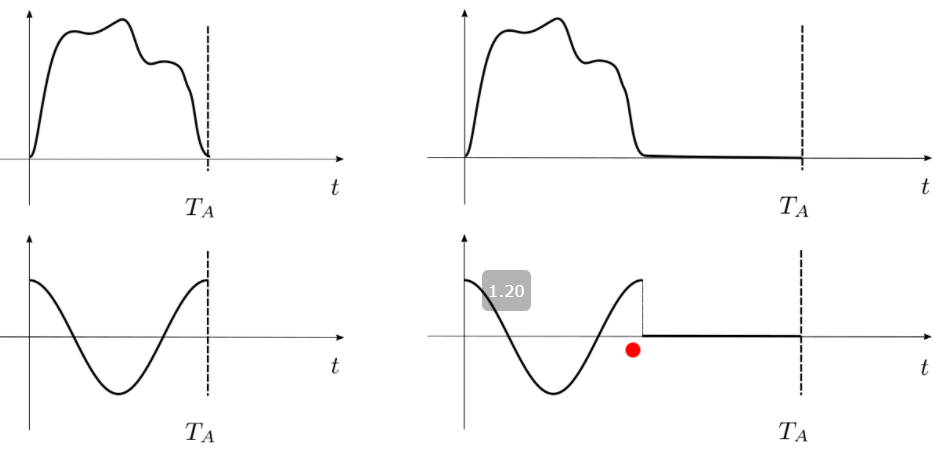
\includegraphics[height =5cm]{Pictures/ZeroPadding.png} 
 \end{itemize}

 \noindent  \\ \textbf{Gewichtetes Fenstern}
\\ Um dem Leakage-Effekt mit nur geringen Nebenwirkungen zu reduzieren, werden Gewichtsfunktionen auf das Zeitsignal angewandt, eine sog. gewichtete Fensterung.\\

 \noindent Dies wird dadurch erreicht, dass man das Originalsignal mit einer Gewichtsfunktion mutlipliziert, 
 bei der am Intervallrand (bei $0$ und $N-1$) die Zeitwerte zur Null gedrückt werden und andererseits kaum neue künstliche Frequenzen eingeführt werden, 
 d.h. die Gewichtsfunktion dazwischen einen möglichst gleichmässigen Verlauf hat in dem das Originalsignal sinnvoll repräsentiert wird: 
 $$x' [n] := w[n] \cdot x[n],\ for n = {0,..nN-1},$$ mit der Gewichtsfunktion $w[n]$.\\

\noindent Hanning-Window:
$$w[n] := 0.5 - 0.5 \cos\bigg(\frac{2\pi n}{N}\bigg)$$
 Blackman-Window:
$$w[n] := 0.42 - 0.5 \cos\bigg(\frac{2\pi n}{N}\bigg) + 0.08 \cos\bigg(\frac{4\pi n}{N}\bigg)$$ 

 \noindent Beispiel: \\
 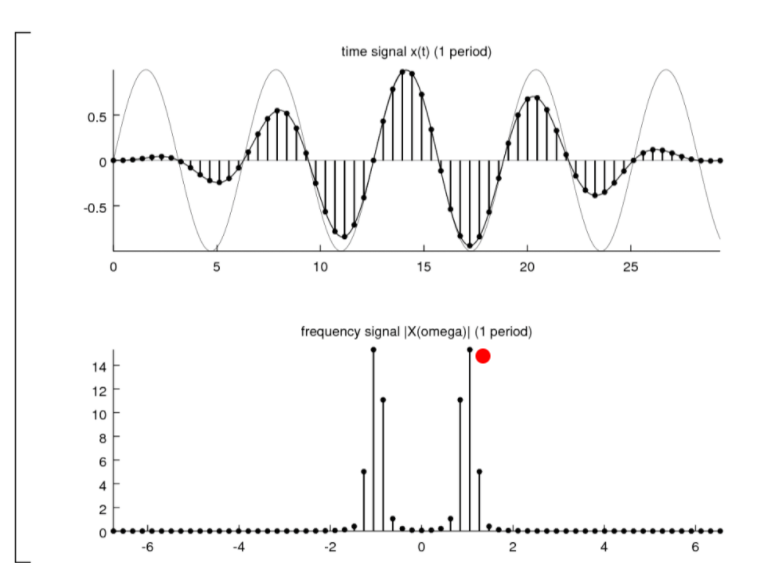
\includegraphics[height=10cm]{Pictures/WeightedWindow.png}

 \subsubsection{Einschub: Die diskrete Faltung}
  \label{sec:sub:sub:diskrete-faltung}

  \noindent \textbf{Azyklische diskrete Faltung:}
  \begin{equation}
    \label{eq:22}
      \begin{split}
      y[n] := x_1[n] * x_2[n] &= \sum_{k=-\infty}^{\infty} x_1[k] \cdot x_2[n-k] \\
      &= \sum_{k=-\infty}^{\infty} x_1 [n-k] \cdot x_2[k]
      \end{split}
    \end{equation}

    \noindent \textbf{Zyklische diskrete Faltung:}
  \begin{equation}
    \label{eq:23}
      \begin{split}
      y[n] := x_P[n] * h[n] &= \sum_{k=0}^{N-1} x_p[n-k] \cdot h_p[k] \\
      \end{split}
    \end{equation}
    Im Normalfalll wählt man die Funktionen $h[n]$ mit $h[n] = 0$ ausserhalb des Grundintervalls $[0, N-1]$, sodass die Periodisierung mit $h_p[n]$ einfach nur eine Wiederholung der Werte des Grundintervalls darstellt und $h_p[k]$ einfach mit $h[k]$ ersetzt werden kann. \\

    \noindent  \textbf{Bemerkungen:}
    \begin{itemize}
      \item Mit der Einführung des diskreten Delta-Impulses $$ \delta [n] =  \begin{cases} 1 &, n = 0 \\ 0 &, n \neq 0 \end{cases} $$
      gibt es analog zu der Faltung mit analogen Signalen die Neutralitätseigenschaft der Faltung: $$ x[n] * \delta [n-n_0] = x[n - n_0]$$
      \item Wenn man mit der DFT arbeitet (und somit mit diskreten und periodischen Signalen) nimmt man die Periodisierung des Zeitsignals $x[n]$ in Kauf, um ein diskretes Spektrum $X[n]$ z uerhalten, 
      jedoch schränkt man sich in der Betrachtung naturgemäss nur auf das Grundintervall $[0, N-1]$ ein und ignoriert die Periodizität 
      von $x[n]$ ausserhalb dieses Grundintervalls. \\
      Bei der diskreten Faltung eines solchen Signals kann jedoch sehr einfach ein Überpsrechen von benachbarten Perioden stattfinden, 
      welches unerwünscht ist aber mit $zero-padding$ vermieden werden kann: \\ 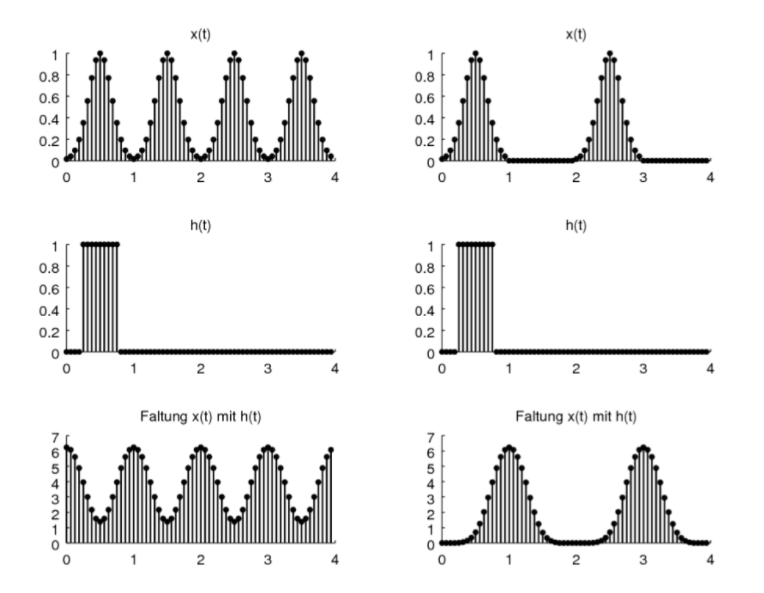
\includegraphics[height = 8cm, width = 15cm]{Pictures/DiskreteFaltung.png}
    \end{itemize}

    \noindent  Herleitung: \\
    \noindent \underline{Azyklische diskrete Faltung $\to$ Zyklische diskrete Faltung} \\
    \noindent Für die digitale Verarbeitung stört das $\infty$ in der Summe der Azyklischen diskreten Faltung. Sind die zu verarbeitenden Signale aber diskret und periodisch so ist möglich: \\

    \noindent Betrachtet man das diskrete und periodische Signal $x_p[n]$ mit Periodendauer $N$, sowie ein allgemeines (nicht-periodisches) Signal $h[n]$. 
    Für diesen Fall gilt mit der Definition der diskreten Faltung und der Aufteilung der Faltungssumme in Teilsummen: 
    \begin{equation}
      \label{eq:24}
        \begin{split}
        y[n] &:= x_P[n] * h[n] \\
        y[n] &= \sum_{k=-\infty}^{\infty} x_P[n-k] \cdot h[k] \\
        y[n] &= ... \sum_{k=-N}^{-1} x_P[n-k] \cdot h[k] +\\
        &+ \sum_{k=0}^{N-1} x_P[n-k] \cdot h[k] + ...\\
        \end{split}
      \end{equation}
      \noindent Bringt man die Summen über Indexverschiebung zu den gleichen Summengrenzen:
      \begin{equation}
        \label{eq:25}
          \begin{split}
          y[n] &= ... \sum_{k=0}^{N-1} x_P[n-k + N] \cdot h[k - N] + \\
          &  +  \sum_{k=0}^{N-1} x_P[n-k] \cdot h[k] + ...\\
          y[n] &= \sum_{k=0}^{N-1} \sum_{l = -\infty}^{\infty} x_p [n -k -l \cdot N] \cdot h[k + l\cdot N]
          \end{split}
        \end{equation}
\noindent Einerseits gilt wegen der Periodizität $x_p[n-k -l\cdot N] = x_p[n-k]$ und somit
$$y[n] = \sum_{k=0}^{N-1} x_p[n-k]\cdot \sum_{l=-\infty}^{\infty} h[k + l\cdot N]$$
und andererseits, stellt 
$$h_p [k] := \sum_{l=-\infty}^{\infty} h[k + l\cdot N]$$
eine periodisierte Version von $h[k]$ dar mit $h_p[k + v\cdot N] = h_p[k]$ für alle $v \in \mathbb{Z}$.

\noindent Mit dieser Definition ergibt sich die Faltung zu einer endlichen Summe bzw. zur zyklischen diskreten Faltung (verweis auf \ref{eq:23}).

\subsubsection{Besonderheiten der DFT}
  \label{sec:sub:sub:besonderheiten-dft}

  \noindent \textbf{Eigenschaften der CTFT:}\\
  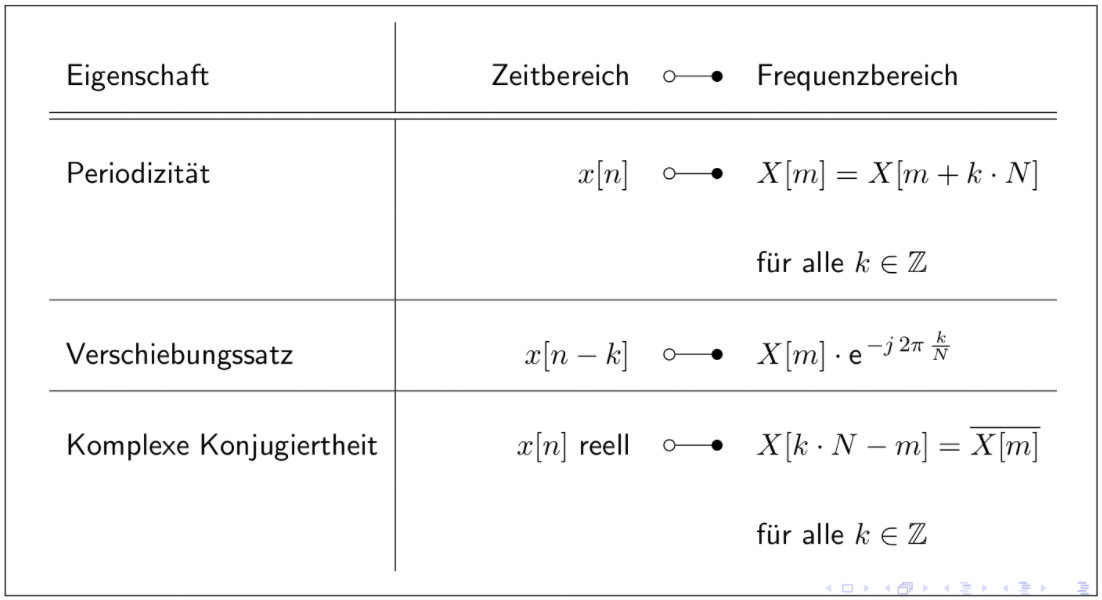
\includegraphics[height = 8cm]{Pictures/EigenschaftenDFT.png}\\
  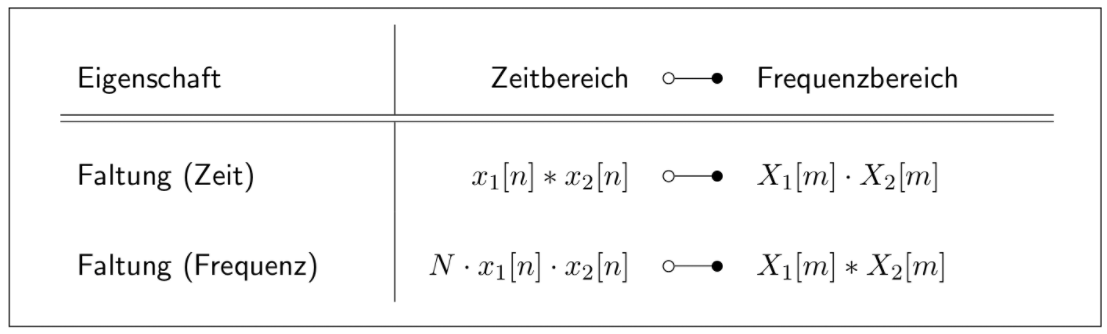
\includegraphics[height = 4.5cm]{Pictures/EigenschaftenDFT2.png}\\

  \newpage       
\end{document}